% ============================================================
%  Semana 10 · Clase 19: De la analítica descriptiva a la predictiva
%  Curso: Análisis y Visualización de Datos para la Toma de Decisiones
%
%  Formato de la sesión (3 h):
%    Hora 1. Descripción, diagnóstico y predicción; variable objetivo y
%            variables explicativas; correlación y causalidad
%    Hora 2. Idea general del Machine Learning supervisado; entrenamiento
%            y prueba; selección y extracción de características
%    Hora 3. Herramientas (Orange, KNIME, RapidMiner, Weka, Python) con
%            sus pros y contras; actividad: formular una pregunta
%            predictiva y seleccionar variables
%
%  Las cifras de los ejemplos salen de datos/gimnasio_vitalis.xlsx (Clases
%  13 a 15), con los 300 socios sin duplicados y fecha de corte 2026-09-30.
%
%  Compilar (dos veces) directamente desde esta carpeta:
%    xelatex semana10-clase19.tex
%    xelatex semana10-clase19.tex
% ============================================================
\documentclass[aspectratio=169,11pt]{beamer}

\usepackage{../../../plantilla/beamerthemeesumer}
\usetheme{esumer}

\usepackage[spanish,es-noshorthands]{babel}
\usepackage{booktabs}
\usepackage{graphicx}
\usepackage{array}
\newcolumntype{L}[1]{>{\raggedright\arraybackslash}p{#1}}
\newcolumntype{C}[1]{>{\centering\arraybackslash}p{#1}}
\usetikzlibrary{arrows.meta,positioning,calc,decorations.pathreplacing,shapes.geometric}

% ---------------- DATOS DE LA CLASE ----------------
\title{De la analítica descriptiva a la predictiva}
\subtitle{Del qué pasó al qué va a pasar}
\author{Docente: Cristian A. Jimenez C., MSc}
\date{Nov 10 al 15}

\setmodulo{Módulo 4: Innovar (Analítica Predictiva y Storytelling)}
\setsemana{10}
\setclase{19}
\setfechaclase{Nov 10 al 15}
\setmodalidad{Virtual}
% -----------------------------------------------------

\graphicspath{{figuras/}}

% Código en un recuadro sin título
\newcommand{\codigo}[1]{\par\smallskip\noindent\colorbox{esumerGray!70}{\parbox{\dimexpr\linewidth-2\fboxsep\relax}{\scriptsize\ttfamily #1}}\par\smallskip}

% Enlace al sitio oficial, al pie de una diapositiva
\newcommand{\sitio}[2]{%
  \par\vspace{1pt}{\fontsize{6}{7}\selectfont\color{black!55}%
  Sitio oficial: \href{#2}{\color{esumerOrange}#1}.\par}}

% Pros y contras de una herramienta
\newcommand{\pro}{\item[{\color{esumerGreen!80!black}\textbf{+}}]}
\newcommand{\contra}{\item[{\color{esumerOrange}\textbf{--}}]}

\newcommand{\urlorange}{https://orangedatamining.com/download/}
\newcommand{\urlorangerank}{https://orangedatamining.com/widget-catalog/data/rank/}
\newcommand{\urlknime}{https://www.knime.com/downloads}
\newcommand{\urlknimecorr}{https://hub.knime.com/knime/extensions/org.knime.features.base/latest/org.knime.base.node.preproc.correlation.filter.CorrelationFilterNodeFactory}
\newcommand{\urlrapid}{https://www.siemens.com/en-us/products/rapidminer/ai-studio/}
\newcommand{\urlrapidcorr}{https://docs.rapidminer.com/latest/studio/operators/modeling/feature_weights/weight_by_correlation.html}
\newcommand{\urlweka}{https://waikato.github.io/weka-wiki/downloading_weka/}
\newcommand{\urlcolab}{https://colab.research.google.com/}
\newcommand{\urlsklearnsel}{https://scikit-learn.org/stable/modules/feature_selection.html}
\newcommand{\urlsklearnpca}{https://scikit-learn.org/stable/modules/decomposition.html}
\newcommand{\urlspurious}{https://tylervigen.com/spurious-correlations}
\newcommand{\urlspuriousA}{https://tylervigen.com/spurious/correlation/5920_per-capita-consumption-of-margarine_correlates-with_the-divorce-rate-in-maine}
\newcommand{\urlspuriousB}{https://tylervigen.com/spurious/correlation/2203_yogurt-consumption_correlates-with_google-searches-for-i-cant-even}
\newcommand{\urlsplit}{https://scikit-learn.org/stable/modules/generated/sklearn.model_selection.train_test_split.html}

\begin{document}

{
\setbeamertemplate{footline}{}
\begin{frame}[plain,noframenumbering]
  \titlepage
\end{frame}
}

\begin{frame}[t]{Agenda de hoy (3 horas)}
  \begin{columns}[T,onlytextwidth]
    \column{0.32\textwidth}
    \begin{block}{Hora 1}
      \small De describir a predecir: variable objetivo, variables
      explicativas, correlación y causalidad.
    \end{block}
    \column{0.32\textwidth}
    \begin{block}{Hora 2}
      \small Cómo aprende un modelo: tareas supervisadas, entrenamiento y
      prueba, y cómo elegir y crear sus características.
    \end{block}
    \column{0.32\textwidth}
    \begin{block}{Hora 3}
      \small Gini, entropía y $\chi^2$ con los datos del gimnasio;
      herramientas con sus pros y contras, y la actividad.
    \end{block}
  \end{columns}
  \vspace{0.3cm}
  \small Hasta ahora contaste \textbf{qué pasó} y \textbf{por qué}: el 80\%
  de los socios del gimnasio sigue activo, y los que viven lejos se retiran
  más. Hoy damos el paso siguiente: usar esos datos para \textbf{anticipar
  qué va a pasar}. En la Clase 20 lo harás con Python.
\end{frame}

\begin{frame}[t]{Palabras nuevas de hoy}
  \footnotesize
  \renewcommand{\arraystretch}{1.1}
  \begin{tabular}{@{}L{3.6cm}L{9.9cm}@{}}
    \toprule
    \textbf{Variable objetivo} & Lo que quieres predecir. También se llama \textit{target} o $y$. Ejemplo: si el socio sigue activo. \\
    \textbf{Variables explicativas} & Lo que usas para predecir. También se llaman \textit{características}, \textit{features} o $X$. Ejemplo: distancia a la sede, plan. \\
    \textbf{Modelo} & Una regla aprendida de los datos que, con las variables explicativas, da una predicción. \\
    \textbf{Clasificación y regresión} & Las dos tareas supervisadas: predecir una categoría (activo o no) o un número (cuántas visitas). \\
    \textbf{Entrenamiento y prueba} & Los datos con que el modelo aprende, y los que se guardan aparte para comprobar si acierta con casos que no vio. \\
    \textbf{Sobreajuste} & Cuando el modelo memoriza los casos de entrenamiento y falla con los nuevos. \\
    \textbf{Selección de características} & Elegir qué columnas entran al modelo y cuáles no. \\
    \textbf{Extracción de características} & Crear columnas nuevas, más útiles, a partir de las que tienes. \\
    \textbf{Fuga de información} & Usar sin querer un dato que delata la respuesta y que no tendrías al momento de predecir (en inglés, \textit{data leakage}). \\
    \bottomrule
  \end{tabular}
\end{frame}

% ============================================================
\section{Hora 1: De describir a predecir}
% ============================================================
\begin{frame}[t]{Cuatro preguntas, cuatro tipos de analítica}
  \small
  Cada tipo responde una pregunta distinta sobre los mismos datos. Las dos
  primeras ya las hiciste en los Módulos 2 y 3.
  \vspace{0.15cm}
  \begin{center}
  \begin{tikzpicture}[
    esc/.style={draw=none, rounded corners=3pt, text=white, align=center,
                minimum width=3.15cm, text width=2.95cm, inner sep=4pt, font=\footnotesize},
    ej/.style={draw=esumerNavy!40, rounded corners=2pt, fill=white, align=left,
               text width=2.95cm, inner sep=4pt, font=\scriptsize, anchor=north},
  ]
    \node[esc, fill=esumerSky, minimum height=1.1cm] (a) at (1.6,0) {\textbf{Descriptiva}\\¿Qué pasó?};
    \node[esc, fill=esumerTeal, minimum height=1.1cm] (b) at (5.1,0.45) {\textbf{Diagnóstica}\\¿Por qué pasó?};
    \node[esc, fill=esumerOrange, minimum height=1.1cm] (c) at (8.6,0.9) {\textbf{Predictiva}\\¿Qué va a pasar?};
    \node[esc, fill=esumerMagenta, minimum height=1.1cm] (d) at (12.1,1.35) {\textbf{Prescriptiva}\\¿Qué debemos hacer?};
    \node[ej] at (1.6,-0.7) {240 de 300 socios siguen activos (80,0\%).\\[2pt]\textit{Tarjetas, barras (Clase 14).}};
    \node[ej] at (5.1,-0.25) {A menos de 6 km sigue activo el 88,0\%; a 6 km o más, el 61,5\%.\\[2pt]\textit{Comparar grupos (Clase 14).}};
    \node[ej] at (8.6,0.2) {¿Qué socios nuevos tienen más riesgo de retirarse?\\[2pt]\textit{Hoy y Clase 20.}};
    \node[ej] at (12.1,0.65) {¿A quién llamamos esta semana, y con qué oferta?\\[2pt]\textit{Fuera del alcance del curso.}};
    \draw[-{Stealth[length=2.4mm]}, line width=1pt, color=esumerNavy] (0,-2.75) -- (13.9,-2.75)
      node[pos=0.5, below, font=\scriptsize, text=esumerNavy] {más valor para decidir, y también más supuestos y más riesgo de equivocarse};
  \end{tikzpicture}
  \end{center}
\end{frame}

\begin{frame}[t]{Variable objetivo y variables explicativas}
  \small
  Un problema predictivo empieza por separar las columnas en dos grupos:
  \vspace{0.1cm}
  \begin{center}
  \begin{tikzpicture}[
    col/.style={draw=esumerNavy!60, fill=white, minimum width=1.75cm, minimum height=0.55cm,
                font=\scriptsize\ttfamily, inner sep=1pt},
    obj/.style={col, fill=esumerOrange!20, draw=esumerOrange},
  ]
    \foreach \x/\n in {0/distancia, 1.8/plan, 3.6/edad, 5.4/sexo, 7.2/visitas}
      {\node[col] at (\x,0) {\n};}
    \node[font=\scriptsize] at (8.65,0) {\ldots};
    \node[obj] at (10.3,0) {activo};
    \foreach \y/\a/\b/\c/\d/\e/\f in {-0.55/{2,1}/Trimestral/28/F/69/No, -1.1/{0,2}/Mensual/69/M/68/Sí, -1.65/{0,6}/Anual/54/F/74/Sí}
      {\node[col, font=\scriptsize] at (0,\y) {\a};
       \node[col, font=\scriptsize] at (1.8,\y) {\b};
       \node[col, font=\scriptsize] at (3.6,\y) {\c};
       \node[col, font=\scriptsize] at (5.4,\y) {\d};
       \node[col, font=\scriptsize] at (7.2,\y) {\e};
       \node[obj, font=\scriptsize] at (10.3,\y) {\f};}
    \draw[decorate, decoration={brace, amplitude=5pt, mirror}, line width=0.8pt, esumerNavy]
      (-0.85,-2.05) -- (8.05,-2.05) node[midway, below=6pt, font=\footnotesize, text=esumerNavy]
      {\textbf{Variables explicativas ($X$)}: lo que sabes de cada socio};
    \draw[decorate, decoration={brace, amplitude=5pt, mirror}, line width=0.8pt, esumerOrange]
      (9.45,-2.05) -- (11.15,-2.05) node[midway, below=6pt, font=\footnotesize, text=esumerOrange, align=center]
      {\textbf{Objetivo ($y$)}};
  \end{tikzpicture}
  \end{center}
  \vspace{-0.1cm}
  \footnotesize
  \begin{itemize}
    \footnotesize
    \item Cada \textbf{fila} es un caso: aquí, un socio. Siempre define qué
      es una fila antes de empezar.
    \item El objetivo debe estar \textbf{registrado en el pasado}: el
      modelo aprende de socios de los que ya sabemos si se quedaron.
  \end{itemize}
  {\scriptsize\color{black!60}Tres socios reales del archivo del gimnasio
  (\texttt{id\_socio} 38, 12 y 46): distancia en km, edad al 30 de septiembre
  de 2026 y visitas registradas.}
\end{frame}

\begin{frame}[t]{Cómo formular una pregunta predictiva}
  \small
  Una buena pregunta predictiva se puede escribir con esta plantilla:
  \vspace{0.1cm}
  \begin{center}
  \begin{tikzpicture}[
    pz/.style={draw=none, rounded corners=3pt, text=white, align=center, font=\scriptsize,
               minimum height=1.25cm, text width=2.35cm, inner sep=3pt},
  ]
    \node[pz, fill=esumerNavy] (a) at (1.25,0) {\textbf{Para decidir}\\qué haremos};
    \node[pz, fill=esumerOrange] (b) at (4.05,0) {\textbf{quiero predecir}\\el objetivo};
    \node[pz, fill=esumerTeal] (c) at (6.85,0) {\textbf{de cada}\\unidad (la fila)};
    \node[pz, fill=esumerSky] (d) at (9.65,0) {\textbf{usando}\\lo que sé en ese momento};
    \node[pz, fill=esumerMagenta] (e) at (12.45,0) {\textbf{con anticipación}\\de cuánto tiempo};
  \end{tikzpicture}
  \end{center}
  \begin{exampleblock}{Ejemplo con el gimnasio}
    \small \textbf{Para decidir} a qué socios nuevos llamar en su primer
    mes, \textbf{quiero predecir} si seguirán activos \textbf{de cada} socio
    recién inscrito, \textbf{usando} su plan, su edad y la distancia de su
    casa a la sede, \textbf{con anticipación} de unos meses antes de que
    venza su plan.
  \end{exampleblock}
  \footnotesize La última parte es la que más se olvida: si predices el
  día en que el socio ya se fue, la predicción no sirve para nada.
\end{frame}

\begin{frame}[t]{Correlación no es causalidad}
  \small
  Que dos variables se muevan juntas no prueba que una cause la otra.
  Para \textbf{predecir}, la relación basta; para \textbf{decidir qué
  cambiar}, no.
  \vspace{0.1cm}
  \footnotesize
  \renewcommand{\arraystretch}{1.25}
  \begin{tabular}{@{}L{3.3cm}L{4.2cm}L{5.6cm}@{}}
    \toprule
    \textbf{Relación en los datos} & \textbf{¿Sirve para predecir?} & \textbf{¿Prueba una causa?} \\
    \midrule
    Plan Anual: 96,2\% activos. Plan Mensual: 77,9\%. & Sí, es una pista útil. & No: un plan anual casi no alcanza a vencer dentro de un año de datos (Clase 14). \\
    A 6 km o más, 61,5\% activos. A menos de 6 km, 88,0\%. & Sí, y se conoce desde la inscripción. & Tampoco del todo: puede ser la distancia, o algo que va con ella, como el tráfico o el horario de trabajo. \\
    \bottomrule
  \end{tabular}
  \vspace{0.15cm}
  \begin{alertblock}{Tres explicaciones antes de hablar de causa}
    \footnotesize \textbf{Azar} (pocos casos: el plan Semestral tiene solo
    10 socios), \textbf{una tercera variable} que mueve a las dos, o
    \textbf{causa al revés}. Para probar una causa hace falta un
    experimento, por ejemplo una oferta a un grupo y no a otro.
  \end{alertblock}
\end{frame}

\begin{frame}[t]{Correlaciones absurdas, pero casi perfectas}
  \begin{columns}[T,onlytextwidth]
    \column{0.49\textwidth}
    \centering
    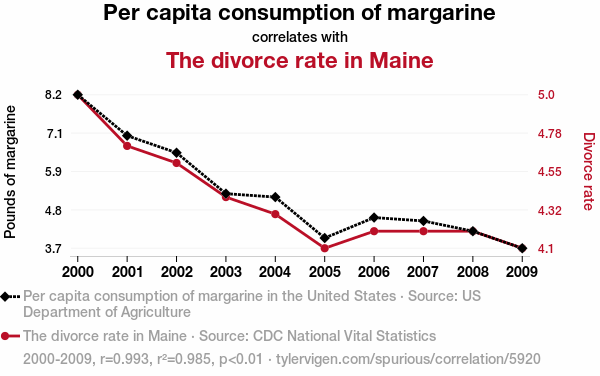
\includegraphics[width=\linewidth,height=3.9cm,keepaspectratio]{spurious/5920.png}\\[1pt]
    {\scriptsize Consumo de margarina en EE.\,UU. y tasa de divorcios en
    Maine, 2000 a 2009: $r = 0{,}993$.}
    \column{0.49\textwidth}
    \centering
    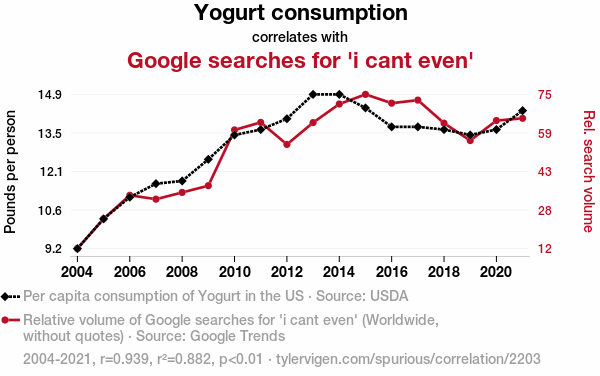
\includegraphics[width=\linewidth,height=3.9cm,keepaspectratio]{spurious/2203.png}\\[1pt]
    {\scriptsize Consumo de yogur en EE.\,UU. y búsquedas en Google de
    ``i cant even'', 2004 a 2021: $r = 0{,}939$.}
  \end{columns}
  \vspace{0.12cm}
  \footnotesize
  \textbf{¿Por qué salen tan altas?} \textbf{(1)} Las dos series
  \textbf{cambian con el tiempo}: casi todo lo que sube o baja año tras año se
  ``correlaciona''. \textbf{(2)} El autor cruzó \textbf{millones de pares} de
  variables y muestra las que coinciden por azar. \textbf{(3)} El
  \textbf{doble eje} (Clase 11) se ajusta para que las líneas se encimen.
  Un modelo que use la margarina para predecir divorcios acertaría en esos
  años y fallaría en los siguientes.
  \par\vspace{1pt}{\fontsize{5.5}{6.5}\selectfont\color{black!55}%
  Gráficas sin modificar de Tyler Vigen,
  \href{\urlspurious}{\color{esumerOrange}Spurious Correlations}
  (correlaciones \href{\urlspuriousA}{\color{esumerOrange}5920} y
  \href{\urlspuriousB}{\color{esumerOrange}2203}), licencia
  \href{https://creativecommons.org/licenses/by/4.0/}{\color{esumerOrange}CC BY 4.0}.\par}
\end{frame}

% ============================================================
\section{Hora 2: Cómo aprende un modelo}
% ============================================================
\begin{frame}[t]{La idea del Machine Learning supervisado}
  \small
  ``Supervisado'' significa que aprende de ejemplos \textbf{con la respuesta
  conocida}, como un estudiante que practica con ejercicios resueltos.
  \vspace{0.2cm}
  \begin{center}
  \begin{tikzpicture}[
    bx/.style={draw=esumerNavy, line width=0.7pt, rounded corners=3pt, fill=white,
               align=center, font=\scriptsize, text width=2.5cm, minimum height=1.35cm},
    fl/.style={-{Stealth[length=2.2mm]}, line width=0.9pt, color=esumerNavy},
  ]
    \node[bx, fill=esumerBg] (h) at (0,0) {\textbf{Historia}\\socios con $X$\\y con $y$ conocida};
    \node[bx, fill=esumerTeal!20] (a) at (3.5,0) {\textbf{Algoritmo}\\busca el patrón entre $X$ y $y$};
    \node[bx, fill=esumerOrange!20] (m) at (7,0) {\textbf{Modelo}\\la regla aprendida};
    \node[bx] (n) at (7,-2.0) {\textbf{Socio nuevo}\\solo con $X$};
    \node[bx, fill=esumerNavy, text=white] (p) at (10.6,-1.0) {\textbf{Predicción}\\``riesgo alto de retirarse''};
    \draw[fl] (h) -- (a);
    \draw[fl] (a) -- (m);
    \draw[fl] (m.east) -| ($(p.north)+(-0.4,0)$);
    \draw[fl] (n.east) -| ($(p.south)+(-0.4,0)$);
  \end{tikzpicture}
  \end{center}
  \vspace{0.05cm}
  \footnotesize
  \begin{itemize}
    \footnotesize
    \item El modelo no ``sabe'' por qué se retira la gente: encuentra
      patrones que se repitieron en el pasado.
    \item Si el futuro cambia (una sede nueva, una competencia), el patrón
      puede dejar de valer. Por eso se vuelve a revisar.
  \end{itemize}
\end{frame}

\begin{frame}[t]{Las tareas supervisadas}
  \small
  La variable objetivo $y$ decide la tarea: si es una categoría,
  clasificación; si es un número, regresión. Las dos predicen.
  \vspace{0.1cm}
  \begin{center}
  \begin{tikzpicture}[
    raiz/.style={draw=none, rounded corners=3pt, fill=esumerNavy, text=white, align=center,
                 font=\footnotesize, text width=5.2cm, inner sep=4pt},
    tipo/.style={draw=none, rounded corners=3pt, text=white, align=center,
                 font=\footnotesize, text width=4.6cm, inner sep=4pt},
    hoja/.style={draw=esumerNavy!50, rounded corners=2pt, fill=white, align=left,
                 font=\scriptsize, text width=3.1cm, inner sep=3pt, anchor=north,
                 execute at begin node={\hyphenpenalty=10000}},
    fl/.style={-{Stealth[length=2mm]}, line width=0.8pt, color=esumerNavy},
  ]
    \node[raiz] (r) at (6.9,0) {\textbf{Aprendizaje supervisado}\\los ejemplos traen la $y$ conocida};
    \node[tipo, fill=esumerTeal] (c) at (3.4,-1.35) {\textbf{Clasificación}: $y$ es una categoría};
    \node[tipo, fill=esumerOrange] (g) at (10.4,-1.35) {\textbf{Regresión}: $y$ es un número};
    \node[hoja] (c1) at (1.65,-2.1) {\textbf{Binaria}: dos clases.\\¿El socio seguirá activo? (Sí / No)};
    \node[hoja] (c2) at (5.15,-2.1) {\textbf{Multiclase}: tres o más.\\¿Qué plan elegirá? (Mensual, Trimestral, Semestral, Anual)};
    \node[hoja] (g1) at (8.65,-2.1) {\textbf{Regresión}: un número.\\¿Cuántas visitas hará el socio el próximo mes?};
    \node[hoja] (g2) at (12.15,-2.1) {\textbf{Pronóstico}: el número a lo largo del tiempo.\\¿Cuánto venderá cada cafetería en diciembre?};
    \draw[fl] (r.south) -- ++(0,-0.3) -| (c.north);
    \draw[fl] (r.south) -- ++(0,-0.3) -| (g.north);
    \draw[fl] (c.south) -- ++(0,-0.15) -| (c1.north);
    \draw[fl] (c.south) -- ++(0,-0.15) -| (c2.north);
    \draw[fl] (g.south) -- ++(0,-0.15) -| (g1.north);
    \draw[fl] (g.south) -- ++(0,-0.15) -| (g2.north);
  \end{tikzpicture}
  \end{center}
  \vspace{-0.1cm}
  \begin{block}{¿Y si no hay $y$?}
    \footnotesize Es aprendizaje \textbf{no supervisado}: por ejemplo,
    agrupar a los socios en segmentos parecidos sin decirle al modelo qué
    buscar. No hay respuesta correcta con qué comparar, y no es tema de
    este curso.
  \end{block}
\end{frame}

\begin{frame}[t]{Las dos tareas, en un dibujo}
  \begin{columns}[T,onlytextwidth]
    \column{0.49\textwidth}
    \centering
    {\small\bfseries\color{esumerTeal} Clasificación: ¿de qué lado cae?}\\[2pt]
    \begin{tikzpicture}[x=0.85cm, y=0.85cm,
      act/.style={circle, fill=esumerTeal, inner sep=0pt, minimum size=4.2pt},
      ina/.style={regular polygon, regular polygon sides=3, fill=esumerOrange, inner sep=0pt, minimum size=6.5pt},
    ]
      \fill[esumerTeal!8] (0,0) -- (0,3.6) -- (2.2,3.6) .. controls (2.8,2.2) and (4.2,1.6) .. (6.0,1.3) -- (6.0,0) -- cycle;
      \fill[esumerOrange!8] (2.2,3.6) .. controls (2.8,2.2) and (4.2,1.6) .. (6.0,1.3) -- (6.0,3.6) -- cycle;
      \draw[esumerNavy, dashed, line width=1pt] (2.2,3.6) .. controls (2.8,2.2) and (4.2,1.6) .. (6.0,1.3);
      \draw[-{Stealth[length=2mm]}, esumerNavy] (0,0) -- (6.2,0) node[below left, font=\scriptsize, text=black] {característica 1};
      \draw[-{Stealth[length=2mm]}, esumerNavy] (0,0) -- (0,3.8) node[above right, font=\scriptsize, text=black] {característica 2};
      \foreach \p in {(0.5,0.6),(0.9,1.5),(1.3,0.4),(1.6,2.2),(0.6,2.8),(2.1,1.1),(2.6,0.5),(1.2,3.1),(3.1,0.9),(3.6,0.4),(2.4,1.8),(0.3,1.9),(1.9,2.9),(2.9,0.2)}
        {\node[act] at \p {};}
      \foreach \p in {(3.4,2.6),(4.1,3.1),(4.8,2.2),(5.5,2.9),(3.0,3.3),(5.6,2.0),(3.9,2.3)}
        {\node[ina] at \p {};}
      \node[circle, draw=esumerNavy, line width=1pt, fill=white, inner sep=0pt, minimum size=9pt, font=\tiny\bfseries] (n) at (3.5,1.25) {?};
      \draw[<-, esumerNavy] (n.south east) -- ++(0.5,-0.35) node[right, font=\scriptsize, text=esumerNavy, align=left] {caso nuevo:\\cae del lado ``activo''};
    \end{tikzpicture}\\[2pt]
    \raggedright\scriptsize
    {\color{esumerTeal}$\bullet$} activos \quad {\color{esumerOrange}$\blacktriangle$} inactivos.
    El modelo aprende una \textbf{frontera} que separa las clases. A un caso
    nuevo le asigna la clase de la zona donde cae.
    \column{0.49\textwidth}
    \centering
    {\small\bfseries\color{esumerOrange} Regresión: ¿qué valor tendrá?}\\[2pt]
    \begin{tikzpicture}[x=0.85cm, y=0.85cm,
      pt/.style={circle, fill=esumerSky, inner sep=0pt, minimum size=4.2pt},
    ]
      \draw[-{Stealth[length=2mm]}, esumerNavy] (0,0) -- (6.2,0) node[below left, font=\scriptsize, text=black] {variable explicativa};
      \draw[-{Stealth[length=2mm]}, esumerNavy] (0,0) -- (0,3.8) node[above right, font=\scriptsize, text=black] {objetivo (un número)};
      \draw[esumerOrange, line width=1.2pt] (0.3,0.55) -- (5.9,3.35);
      \foreach \x/\y in {0.5/0.95, 0.9/0.55, 1.4/1.25, 1.8/0.95, 2.3/1.75, 2.7/1.35, 3.2/2.05, 3.6/1.7, 4.1/2.65, 4.5/2.2, 5.0/3.15, 5.4/2.75}
        {\draw[black!45, line width=0.5pt] (\x,\y) -- (\x,{0.55+(\x-0.3)*0.5});
         \node[pt] at (\x,\y) {};}
      \draw[esumerNavy, dashed] (2.0,0) node[below, font=\scriptsize] {caso nuevo} -- (2.0,1.4) -- (0,1.4) node[left, font=\scriptsize] {predicción};
      \node[circle, draw=esumerNavy, line width=1pt, fill=white, inner sep=0pt, minimum size=7pt] at (2.0,1.4) {};
    \end{tikzpicture}\\[2pt]
    \raggedright\scriptsize
    El modelo aprende una \textbf{línea} (o curva) que sigue la tendencia
    de los puntos. Para un caso nuevo, la predicción es la altura de la
    línea. Las rayas grises son los \textbf{errores}: lo que tendrás que
    medir en la Clase 20.
  \end{columns}
  \vspace{0.12cm}
  {\scriptsize\color{black!60}Esquemas: los puntos no son datos reales; solo muestran la idea de cada tarea.}
\end{frame}

\begin{frame}[t]{Clasificación y regresión: sus diferencias}
  \footnotesize
  \renewcommand{\arraystretch}{1.05}
  \begin{tabular}{@{}L{2.9cm}L{5.1cm}L{5.1cm}@{}}
    \toprule
    & \textbf{Clasificación} & \textbf{Regresión} \\
    \midrule
    \textbf{Pregunta típica} & ¿Cuál? ¿Sí o no? & ¿Cuánto? ¿Cuántos? \\
    \textbf{Qué responde el modelo} & Una clase, o la probabilidad de cada una: ``82\% de seguir activo''. & Un número: ``9 visitas el próximo mes''. \\
    \textbf{Cómo se mide si acierta} & Porcentaje de aciertos, y a cuántos de cada clase encuentra. & Cuánto se equivoca, en las unidades del objetivo, y el $R^2$ (Clase 20). \\
    \textbf{Línea base} & Decir siempre la clase más frecuente: 80\% de aciertos en el gimnasio. & Decir siempre el promedio. \\
    \textbf{Criterios para elegir columnas} & Gini, entropía, $\chi^2$, ANOVA. & Correlación. \\
    \textbf{Modelos típicos} & Regresión logística, árbol de decisión, $k$ vecinos más cercanos. & Regresión lineal (Clase 20), árbol de regresión. \\
    \bottomrule
  \end{tabular}
  \vspace{0.1cm}

  \begin{columns}[T,onlytextwidth]
    \column{0.48\textwidth}
    \scriptsize{\color{esumerOrange}\textbf{Cuidado con el nombre.}} La
    \textbf{regresión logística} es de \textbf{clasificación}: calcula la
    probabilidad de una clase, aunque se llame regresión.
    \column{0.48\textwidth}
    \scriptsize{\color{esumerNavy}\textbf{El pronóstico es especial.}} El
    orden del tiempo importa: se entrena con los meses pasados y se prueba
    con los siguientes, no con un reparto al azar.
  \end{columns}
\end{frame}

\begin{frame}[t]{Entrenamiento y prueba}
  \begin{columns}[T,onlytextwidth]
    \column{0.5\textwidth}
    \small
    \textbf{El examen que el modelo no ha visto.} Si evalúas al modelo con
    los mismos casos con que aprendió, es como
    calificar un examen con las preguntas que el estudiante ya memorizó.
    \vspace{0.15cm}

    \begin{tikzpicture}
      \fill[esumerTeal] (0,0) rectangle (5.2,0.7);
      \fill[esumerOrange] (5.2,0) rectangle (6.5,0.7);
      \node[text=white, font=\scriptsize\bfseries] at (2.6,0.35) {Entrenamiento: 240 socios (80\%)};
      \node[text=white, font=\scriptsize\bfseries, align=center] at (5.85,0.35) {Prueba\\60};
      \node[font=\tiny, text=black!60, anchor=north west] at (0,-0.05) {300 socios del gimnasio, repartidos al azar};
    \end{tikzpicture}
    \vspace{0.1cm}

    \footnotesize
    \begin{enumerate}
      \footnotesize
      \item El modelo aprende \textbf{solo} con el grupo de entrenamiento.
      \item Predice el grupo de prueba como si fueran socios nuevos.
      \item Comparas sus predicciones con lo que de verdad pasó.
    \end{enumerate}
    \column{0.46\textwidth}
    \footnotesize En Python (Clase 20), una sola función hace el reparto:
    \codigo{from sklearn.model\_selection import \\
      \hspace*{1em}train\_test\_split\\[3pt]
      X = socios[["distancia\_sede\_km", "edad"]]\\
      y = socios["activo"]\\[3pt]
      X\_train, X\_test, y\_train, y\_test = \\
      \hspace*{1em}train\_test\_split(X, y,\\
      \hspace*{2em}test\_size=0.2, random\_state=42)}
    \scriptsize\raggedright \texttt{test\_size=0.2} deja el 20\% para la prueba;
    \texttt{random\_state} hace que el reparto sea el mismo cada vez que lo
    ejecutas.
    \begin{alertblock}{Memorizar no es aprender}
      \scriptsize Un modelo que acierta todo en entrenamiento y falla en
      prueba está \textbf{sobreajustado}: se aprendió los casos, no el
      patrón.
    \end{alertblock}
  \end{columns}
\end{frame}

\begin{frame}[t]{Antes de celebrar: la línea base}
  \small
  Compara siempre con no hacer nada. Si el modelo dice ``activo'' para todos los socios, sin mirar ningún dato,
  ya acierta \textbf{240 de 300: el 80\%}. Esa es la \textbf{línea base}.
  \vspace{0.15cm}
  \begin{center}
  \begin{tikzpicture}
    \draw[esumerGray, line width=6pt] (0,0) -- (11,0);
    \draw[esumerNavy, line width=6pt] (0,0) -- (8.8,0);
    \node[font=\scriptsize, anchor=south east] at (8.75,0.2) {línea base: 80\%};
    \draw[esumerOrange, line width=1pt] (8.8,-0.25) -- (8.8,0.25);
    \node[font=\scriptsize, anchor=north] at (0,-0.2) {0\%};
    \node[font=\scriptsize, anchor=north] at (11,-0.2) {100\%};
    \node[font=\scriptsize, text=esumerOrange, anchor=south west] at (8.85,0.2) {aporte del modelo $\rightarrow$};
  \end{tikzpicture}
  \end{center}
  \begin{columns}[T,onlytextwidth]
    \column{0.48\textwidth}
    \begin{block}{Qué significa}
      \footnotesize Un modelo que acierta el 82\% apenas mejora a no
      hacer nada. Pregunta siempre: ¿cuánto mejor que la línea base?
    \end{block}
    \column{0.48\textwidth}
    \begin{block}{Y además}
      \footnotesize Ese 80\% nunca encuentra a un solo socio que se va a
      retirar, que es justo a quien quieres llamar. Hay que mirar también
      a quién acierta, no solo cuántos.
    \end{block}
  \end{columns}
\end{frame}

\begin{frame}[t]{Características: elegir y crear}
  \small
  El modelo solo ve las columnas que le das. Hay dos tareas, y ninguna
  es automática: las dos piden conocer el negocio.
  \vspace{0.15cm}
  \begin{center}
  \begin{tikzpicture}[
    c/.style={draw=esumerNavy!60, fill=white, minimum width=0.62cm, minimum height=1.3cm, inner sep=0pt},
    fl/.style={-{Stealth[length=2.2mm]}, line width=0.9pt, color=esumerNavy},
  ]
    % Selección
    \node[font=\footnotesize\bfseries, text=esumerTeal] at (3.1,1.25) {Selección: quedarse con las útiles};
    \foreach \i in {0,...,5} {\node[c] at (0.35+0.68*\i,0) {};}
    \draw[fl] (4.45,0) -- (5.15,0);
    \foreach \i in {0,1} {\node[c, fill=esumerTeal!40] at (5.55+0.68*\i,0) {};}
    \node[font=\scriptsize, text width=6cm, align=center] at (3.1,-1.1) {De 6 columnas quedan 2. Las demás no se transforman: se dejan por fuera.};
    % Extracción
    \node[font=\footnotesize\bfseries, text=esumerOrange] at (10.9,1.25) {Extracción: crear columnas nuevas};
    \foreach \i in {0,1,2} {\node[c] at (8.55+0.68*\i,0) {};}
    \draw[fl] (10.55,0) -- (11.25,0);
    \node[c, fill=esumerOrange!40, minimum width=0.9cm] at (11.8,0) {};
    \node[font=\scriptsize, text width=5.6cm, align=center] at (10.9,-1.1) {De fecha de nacimiento y fecha de corte sale la edad; de las coordenadas, la distancia.};
  \end{tikzpicture}
  \end{center}
  \vspace{-0.05cm}
  \begin{columns}[T,onlytextwidth]
    \column{0.48\textwidth}
    \begin{block}{Por qué seleccionar}
      \footnotesize Menos columnas: un modelo más fácil de explicar, que
      se equivoca menos con casos nuevos y que necesita menos datos.
    \end{block}
    \column{0.48\textwidth}
    \begin{block}{Por qué extraer}
      \footnotesize El dato crudo casi nunca es la mejor pista: una fecha
      sola dice poco; la antigüedad que sale de ella dice mucho.
    \end{block}
  \end{columns}
\end{frame}

\begin{frame}[t]{La maldición de la dimensionalidad}
  \small
  ¿Por qué no usar todas las columnas? Porque cada columna nueva
  \textbf{multiplica} el espacio que los datos deben llenar.
  \begin{center}
  \begin{tikzpicture}[x=0.15cm, y=0.15cm]
    % 1 variable
    \foreach \i in {0,...,9} {\draw[esumerNavy!60, fill=esumerTeal!35] (\i,0) rectangle ++(1,1);}
    \node[font=\scriptsize, align=center, anchor=north] at (5,-0.4) {\textbf{1 columna}, 10 tramos\\10 casillas\\30 socios por casilla};
    % 2 variables
    \begin{scope}[xshift=4.7cm]
      \foreach \i in {0,...,9} {\foreach \j in {0,...,9} {\draw[esumerNavy!60, fill=esumerTeal!12] (\i,\j-4.5) rectangle ++(1,1);}}
      \node[font=\scriptsize, align=center, anchor=north] at (5,-4.9) {\textbf{2 columnas}\\100 casillas\\3 socios por casilla};
    \end{scope}
    % 3 variables
    \begin{scope}[xshift=9.0cm]
      \foreach \k in {4,3,2,1,0} {\draw[esumerNavy!60, fill=white] (\k*0.5,\k*0.5-4.5) rectangle ++(10,10);}
      \node[font=\scriptsize, align=center, anchor=north] at (6,-4.9) {\textbf{3 columnas}\\1.000 casillas\\0,3 socios por casilla};
    \end{scope}
  \end{tikzpicture}
  \end{center}
  \vspace{-0.1cm}
  \begin{columns}[T,onlytextwidth]
    \column{0.52\textwidth}
    \footnotesize Con \textbf{300 socios} y 10 tramos por columna, con 3
    columnas ya hay más casillas que socios: casi todas quedan
    \textbf{vacías}. El modelo adivina donde nunca vio a nadie y
    \textbf{memoriza} los pocos casos que vio (sobreajuste).
    \column{0.44\textwidth}
    \begin{block}{Qué hacer}
      \footnotesize Seleccionar y extraer: pocas columnas buenas. Regla
      práctica: unos 10 casos de la clase menos frecuente por columna. Con
      60 inactivos, unas 6 columnas.
    \end{block}
  \end{columns}
\end{frame}

\begin{frame}[t]{Extracción: ya lo has hecho en el curso}
  \small
  Cada columna nueva que creaste es una característica extraída:
  \vspace{0.1cm}
  \footnotesize
  \renewcommand{\arraystretch}{1.2}
  \begin{tabular}{@{}L{3.0cm}L{3.2cm}L{4.0cm}L{2.4cm}@{}}
    \toprule
    \textbf{Dato crudo} & \textbf{Característica} & \textbf{Cómo} & \textbf{Dónde} \\
    \midrule
    \texttt{fecha\_nacimiento} & edad & diferencia con la fecha de corte & Clases 8 y 13 \\
    \texttt{fecha\_inscripcion} & días como socio & \texttt{DATEDIFF} o resta de fechas & Clase 14 \\
    latitud y longitud & distancia a la sede, en km & fórmula de distancia entre dos puntos (venía calculada) & Clases 13 y 14 \\
    \texttt{hora\_entrada} & hora del día, franja & \texttt{HOUR}, \texttt{pd.cut} & Clases 8 y 14 \\
    tabla de asistencias & visitas por socio & agrupar y contar (\texttt{groupby}) & Clase 9 \\
    \bottomrule
  \end{tabular}
  \vspace{0.15cm}
  \begin{exampleblock}{Una técnica más: combinar muchas columnas en pocas}
    \footnotesize Cuando hay decenas de columnas numéricas parecidas, el
    \textbf{análisis de componentes principales} (PCA) las resume en unas
    pocas columnas nuevas que conservan casi toda la información. El costo:
    esas columnas nuevas ya no tienen un significado de negocio fácil de
    explicar.
  \end{exampleblock}
\end{frame}

\begin{frame}[t]{Selección: cinco preguntas para cada columna}
  \begin{columns}[T,onlytextwidth]
    \column{0.54\textwidth}
    \small
    \begin{enumerate}
      \small
      \item \textbf{¿La tendré al momento de predecir?} Si no, es fuga de
        información.
      \item \textbf{¿Se relaciona con el objetivo?} Compara activos e
        inactivos, o calcula la correlación.
      \item \textbf{¿Repite lo que dice otra?} Visitas totales y días como
        socio tienen correlación de 0,62: dicen parte de lo mismo.
      \item \textbf{¿Es confiable?} Muchos vacíos o errores la debilitan.
      \item \textbf{¿Es justo y legal usarla?} Sexo, edad u origen pueden
        discriminar, aunque predigan.
    \end{enumerate}
    \column{0.42\textwidth}
    \begin{alertblock}{Fuera desde el inicio}
      \footnotesize Los \textbf{identificadores}: \texttt{id\_socio},
      nombre, correo, teléfono. Son únicos por persona: el modelo los
      memoriza y no aprende nada que sirva para un socio nuevo. Además,
      son datos personales (Clase 1).
    \end{alertblock}
    \begin{block}{Los métodos automáticos}
      \footnotesize Existen métodos que ordenan o prueban combinaciones de
      columnas: por \textbf{filtro} (una medida, como la correlación), por
      \textbf{envoltura} (probar el modelo con distintos grupos) e
      \textbf{integrados} al modelo. Ayudan con la pregunta 2, pero
      ninguno responde la 1 ni la 5.
    \end{block}
  \end{columns}
\end{frame}

\begin{frame}[t]{Selección con los datos del gimnasio}
  \footnotesize
  Promedios de los 240 activos y los 60 inactivos, al 30 de septiembre de 2026:
  \vspace{0.05cm}

  \renewcommand{\arraystretch}{1.1}
  \begin{tabular}{@{}L{3.1cm}C{1.4cm}C{1.4cm}L{6.8cm}@{}}
    \toprule
    \textbf{Columna candidata} & \textbf{Activos} & \textbf{Inactivos} & \textbf{Decisión} \\
    \midrule
    distancia a la sede (km) & 4,3 & 7,4 & \leavevmode{\color{esumerGreen!70!black}\textbf{Entra.}} Hay diferencia y se conoce desde la inscripción. \\
    plan & \multicolumn{2}{C{3.2cm}}{Anual 96,2\%; Mensual 77,9\%} & \leavevmode{\color{esumerGreen!70!black}\textbf{Entra}}, con la advertencia de la diapositiva de causalidad. \\
    edad (años) & 37,4 & 37,5 & \leavevmode{\color{black!60}\textbf{Probablemente no aporta.}} Casi no hay diferencia. \\
    sexo & \multicolumn{2}{C{3.2cm}}{F 79,3\%; M 79,5\%} & \leavevmode{\color{black!60}\textbf{Fuera.}} No hay diferencia, y es un dato sensible. \\
    visitas totales & 62,4 & 35,0 & \leavevmode{\color{esumerOrange}\textbf{Cuidado.}} Los activos llevan más tiempo yendo: es en parte consecuencia de seguir activo. \\
    días sin venir & 3,3 & 68,0 & \leavevmode{\color{esumerOrange}\textbf{Fuera: es fuga.}} Ver la siguiente diapositiva. \\
    \bottomrule
  \end{tabular}
  \vspace{0.1cm}

  \scriptsize Plan y sexo son categorías: se muestra el porcentaje de
  activos de cada grupo. Hay 9 socios sin sexo registrado.
\end{frame}

\begin{frame}[t]{La trampa: una columna que delata la respuesta}
  \begin{columns}[T,onlytextwidth]
    \column{0.5\textwidth}
    \small
    \textbf{Días desde la última visita}, en mediana:
    \vspace{0.1cm}

    \begin{tikzpicture}
      \fill[esumerTeal] (0,0.6) rectangle (0.15,1.1);
      \node[font=\scriptsize, anchor=west] at (0.2,0.85) {Activos: \textbf{1 día}};
      \fill[esumerOrange] (0,-0.2) rectangle (5.55,0.3);
      \node[font=\scriptsize, text=white, anchor=east] at (5.5,0.05) {Inactivos: \textbf{37 días}};
    \end{tikzpicture}
    \vspace{0.1cm}

    \footnotesize Una regla tan simple como ``si lleva más de 30 días sin
    venir, se retiró'' acierta con el \textbf{91\%} de los socios. Supera
    la línea base del 80\%. Parece un gran modelo.
    \column{0.46\textwidth}
    \begin{alertblock}{Pero no sirve}
      \footnotesize Un socio deja de venir \textbf{porque ya se retiró}. Esa
      columna describe la respuesta, no la anticipa. Cuando la tienes, ya
      es tarde para llamarlo.
    \end{alertblock}
    \begin{exampleblock}{La prueba de la fuga}
      \footnotesize Para cada columna pregunta: \textbf{¿la conocería el
      día en que tengo que decidir?} Si la decisión es en el primer mes
      del socio, solo vale lo que se sabe en ese primer mes.
    \end{exampleblock}
  \end{columns}
  \vspace{0.1cm}
  \footnotesize Un resultado demasiado bueno para ser verdad casi siempre es
  una fuga de información.
\end{frame}

\begin{frame}[t]{Criterios para medir cuánto aporta una columna}
  \small
  Los métodos por filtro le ponen un número a cada columna para ordenarlas.
  El criterio depende del tipo de columna y de objetivo:

  \footnotesize
  \renewcommand{\arraystretch}{1.12}
  \begin{tabular}{@{}L{3.0cm}L{5.4cm}L{4.7cm}@{}}
    \toprule
    \textbf{Criterio} & \textbf{Qué mide} & \textbf{Cuándo se usa} \\
    \midrule
    Correlación & Si dos números suben o bajan juntos, en línea recta. & Columna numérica y objetivo numérico (Clase 20). \\
    Índice de Gini & Qué tan \textbf{mezclado} queda cada grupo: 0 si todos son iguales. & Objetivo categórico. Es el criterio de los árboles de decisión. \\
    Entropía y ganancia de información & También la mezcla, medida en bits. La ganancia es cuánto baja la entropía al separar por la columna. & Objetivo categórico. En scikit-learn se llama \textit{información mutua}. \\
    Chi cuadrado ($\chi^2$) & Si la tabla cruzada se aleja de lo que se esperaría si no hubiera relación. Da un \textbf{valor p}. & Columna categórica y objetivo categórico. \\
    ANOVA (prueba F) & Si los promedios de un número cambian entre los grupos del objetivo. & Columna numérica y objetivo categórico. \\
    \bottomrule
  \end{tabular}
  \vspace{0.05cm}

  \scriptsize En Orange, widget \textbf{Rank}. En scikit-learn,
  \texttt{chi2}, \texttt{mutual\_info\_classif} y \texttt{f\_classif}.
\end{frame}

% ============================================================
\section{Hora 3: Criterios y herramientas}
% ============================================================
\begin{frame}[t]{Gini y entropía: ¿se ordena el grupo?}
  \begin{columns}[T,onlytextwidth]
    \column{0.6\textwidth}
    \centering
    \begin{tikzpicture}[
      g/.style={draw=esumerNavy, line width=0.7pt, rounded corners=3pt, fill=white,
                align=center, font=\scriptsize, text width=3.5cm, inner sep=3pt},
      fl/.style={-{Stealth[length=2mm]}, line width=0.8pt, color=esumerNavy},
    ]
      \node[g, fill=esumerBg] (t) at (2.05,0) {\textbf{Todos: 300 socios}\\240 activos (80\%)\\Gini 0,320 \textperiodcentered\ entropía 0,722};
      \node[g, fill=esumerTeal!15] (a) at (0,-2.0) {\textbf{Menos de 6 km: 209}\\184 activos (88,0\%)\\Gini 0,211 \textperiodcentered\ entropía 0,528};
      \node[g, fill=esumerOrange!15] (b) at (4.1,-2.0) {\textbf{6 km o más: 91}\\56 activos (61,5\%)\\Gini 0,473 \textperiodcentered\ entropía 0,961};
      \draw[fl] (t.south) -- ++(0,-0.3) -| (a.north);
      \draw[fl] (t.south) -- ++(0,-0.3) -| (b.north);
    \end{tikzpicture}

    \vspace{0.15cm}
    \raggedright\footnotesize
    Al separar por distancia, el grupo cercano quedó \textbf{más puro} (casi todos activos); el
    lejano, más mezclado. Promediando según el tamaño de cada grupo, el Gini
    baja de 0,320 a 0,290: una \textbf{disminución de 0,030}. La entropía
    baja de 0,722 a 0,660: una \textbf{ganancia de información de 0,062}.
    \column{0.37\textwidth}
    \begin{block}{Las fórmulas}
      \footnotesize $p$ es la proporción de cada clase en el grupo.\\[3pt]
      $\text{Gini} = 1 - \sum p^2$\\[2pt]
      $\text{Entropía} = -\sum p \log_2 p$\\[4pt]
      Para todos los socios:\\
      $1 - (0{,}8^2 + 0{,}2^2) = 0{,}32$
    \end{block}
    \begin{exampleblock}{Cómo se leen}
      \footnotesize 0 es un grupo puro. El máximo (Gini 0,5; entropía 1,
      con dos clases) es mitad y mitad. Una buena columna separa en
      grupos más puros que el original.
    \end{exampleblock}
  \end{columns}
\end{frame}

\begin{frame}[t]{Los tres criterios con los datos del gimnasio}
  \footnotesize
  Objetivo: \texttt{activo}. Edad en tres grupos (menos de 30, 30 a 44, 45 o
  más); sexo, sin los 9 socios que no lo tienen.
  \vspace{0.05cm}

  \renewcommand{\arraystretch}{1.18}
  \begin{tabular}{@{}L{2.5cm}C{2.0cm}C{2.0cm}C{2.2cm}L{3.5cm}@{}}
    \toprule
    \textbf{Columna} & \textbf{Disminución de Gini} & \textbf{Ganancia de información} & \textbf{$\chi^2$ (valor p)} & \textbf{Lectura} \\
    \midrule
    distancia (6 km) & 0,030 & 0,062 & 27,8 (menos de 0,001) & La que más separa. \\
    plan & 0,013 & 0,036 & 12,2 (0,007) & Separa, con menos fuerza. \\
    edad (3 grupos) & 0,003 & 0,008 & 3,1 (0,21) & Sin evidencia de relación. \\
    sexo & 0,000 & 0,000 & 0,0 (0,98) & Ninguna relación. \\
    \bottomrule
  \end{tabular}
  \vspace{0.12cm}

  \begin{columns}[T,onlytextwidth]
    \column{0.48\textwidth}
    \begin{block}{Qué dicen juntos}
      \footnotesize Los tres criterios dan el \textbf{mismo orden}. El valor
      p de $\chi^2$ dice si la relación podría ser azar: por debajo de 0,05,
      es poco probable que lo sea.
    \end{block}
    \column{0.48\textwidth}
    \begin{alertblock}{Lo que no dicen}
      \footnotesize ``Días sin venir'' (más de 30 o no) quedaría
      \textbf{primera} en los tres: Gini baja 0,157 y $\chi^2$ da 146,8.
      Ningún criterio detecta la fuga de información: eso lo decides tú.
    \end{alertblock}
  \end{columns}
\end{frame}

\begin{frame}[t]{Herramientas: de arrastrar cajas a escribir código}
  \small
  Lo que acabas de calcular, y todo lo de la Hora 2, estas herramientas lo
  hacen por ti. Cambia \textbf{cómo} se lo pides.
  \vspace{0.2cm}
  \begin{center}
  \begin{tikzpicture}[
    t/.style={draw=esumerNavy, line width=0.7pt, rounded corners=3pt, fill=white,
              font=\footnotesize\bfseries, minimum width=2.3cm, minimum height=0.8cm, align=center},
  ]
    \shade[left color=esumerTeal!60, right color=esumerOrange!70, rounded corners=2pt] (0,-0.15) rectangle (13.8,0.15);
    \node[font=\scriptsize, anchor=north west, text width=5.2cm, align=left] at (0,-0.3) {\textbf{Visual}: arrastras bloques y los conectas. Sin programar.};
    \node[font=\scriptsize, anchor=north east, text width=5.2cm, align=right] at (13.8,-0.3) {\textbf{Código}: escribes cada paso. Control total.};
    \node[t] at (1.3,1.0) {Orange};
    \node[t] at (4.1,1.0) {Weka};
    \node[t] at (6.9,1.0) {KNIME};
    \node[t, text width=2.3cm, font=\scriptsize\bfseries] at (9.7,1.0) {RapidMiner\\AI Studio};
    \node[t] at (12.5,1.0) {Python};
  \end{tikzpicture}
  \end{center}
  \vspace{0.6cm}
  \footnotesize
  \begin{itemize}
    \footnotesize
    \item En las herramientas visuales, cada caja es un paso (leer el
      archivo, filtrar columnas, entrenar) y las flechas llevan los datos de
      un paso al siguiente. El flujo queda guardado, como los pasos
      aplicados de Power Query.
    \item Ninguna te salva de las preguntas de la Hora 2: todas pueden
      entrenar un modelo con fuga de información si no la detectas tú.
  \end{itemize}
\end{frame}

\begin{frame}[t]{Orange Data Mining}
  \begin{columns}[T,onlytextwidth]
    \column{0.36\textwidth}
    \begin{block}{Qué es}
      \footnotesize Herramienta visual del Laboratorio de Bioinformática de
      la Universidad de Liubliana (Eslovenia). Cada paso es un
      \textbf{widget} que se conecta con otros.\\[3pt]
      \textbf{Licencia}: gratuita y de código abierto (GPL).\\
      \textbf{Equipos}: Windows, macOS y Linux.
    \end{block}
    \footnotesize\textbf{Para características}: los widgets
    \textbf{Rank} (ordena las columnas según cuánto se relacionan con el
    objetivo), \textbf{Select Columns} y \textbf{PCA}.
    \column{0.6\textwidth}
    \footnotesize
    \begin{itemize}
      \footnotesize
      \pro La más fácil para empezar: en minutos tienes un flujo funcionando.
      \pro Gráficos interactivos en cada paso: seleccionas puntos en un
        gráfico y pasan al siguiente widget.
      \pro Muy usada en la enseñanza, con tutoriales en video.
      \pro Complementos para texto, imágenes y otras tareas.
      \contra Pensada para explorar y aprender, no para procesos de la
        empresa que corren solos todos los días.
      \contra Con tablas muy grandes se vuelve lenta.
      \contra Pocos conectores a bases de datos y sistemas empresariales.
    \end{itemize}
  \end{columns}
  \sitio{orangedatamining.com}{\urlorange}
\end{frame}

\begin{frame}[t]{KNIME Analytics Platform}
  \begin{columns}[T,onlytextwidth]
    \column{0.36\textwidth}
    \begin{block}{Qué es}
      \footnotesize Plataforma visual de flujos de trabajo, creada en la
      Universidad de Constanza (Alemania). Cada paso es un
      \textbf{nodo}.\\[3pt]
      \textbf{Licencia}: la plataforma de escritorio es gratuita y de
      código abierto (GPLv3). Compartir y automatizar flujos en servidor
      (KNIME Business Hub) es de pago.\\
      \textbf{Equipos}: Windows, macOS y Linux.
    \end{block}
    \column{0.6\textwidth}
    \footnotesize
    \begin{itemize}
      \footnotesize
      \pro Muy completa: preparar datos, unir fuentes, modelar y reportar
        en un mismo flujo, como un Power Query con modelos.
      \pro Miles de nodos y conectores (Excel, bases de datos, la web).
      \pro Puede ejecutar código de Python o R dentro del flujo.
      \pro Comunidad grande y flujos de ejemplo en KNIME Hub.
      \contra La curva de aprendizaje es mayor que la de Orange: hay tantos
        nodos que cuesta encontrar el correcto.
      \contra Consume bastante memoria del computador.
      \contra Sus gráficos son menos atractivos que los de Orange o Power BI.
    \end{itemize}
    \footnotesize\textbf{Para características}: los nodos
    \textbf{Linear Correlation} y \textbf{Correlation Filter} (quitar
    columnas redundantes), \textbf{Feature Selection Loop} y \textbf{PCA}.
  \end{columns}
  \sitio{knime.com/downloads}{\urlknime}
\end{frame}

\begin{frame}[t]{RapidMiner AI Studio}
  \begin{columns}[T,onlytextwidth]
    \column{0.36\textwidth}
    \begin{block}{Qué es}
      \footnotesize Herramienta visual de ``arrastrar y soltar'' con
      \textbf{operadores}. Nació como RapidMiner; pasó a Altair, que la
      llamó Altair AI Studio, y hoy aparece en el sitio de Siemens.\\[3pt]
      \textbf{Licencia}: comercial. Ha tenido ediciones gratuitas y para
      estudiantes, con condiciones que han cambiado: verifícalas antes de
      adoptarla.
    \end{block}
    \column{0.6\textwidth}
    \footnotesize
    \begin{itemize}
      \footnotesize
      \pro Interfaz guiada, pensada para analistas de negocio.
      \pro Funciones de \textbf{AutoML}: prueba varios modelos por ti y los
        compara.
      \pro Integra cuadernos de Python y R con el flujo visual.
      \pro Muy usada en la industria y en cursos de minería de datos.
      \contra No es software libre: el uso en una empresa requiere licencia.
      \contra Los cambios de dueño y de nombre hacen confusa la
        documentación y las versiones.
      \contra El AutoML tienta a no entender lo que hace el modelo.
    \end{itemize}
    \footnotesize\textbf{Para características}: los operadores
    \textbf{Weight by Correlation}, \textbf{Optimize Selection} (prueba
    combinaciones de columnas) y \textbf{Principal Component Analysis}.
  \end{columns}
  \sitio{siemens.com/en-us/products/rapidminer/ai-studio}{\urlrapid}
\end{frame}

\begin{frame}[t]{Weka}
  \begin{columns}[T,onlytextwidth]
    \column{0.36\textwidth}
    \begin{block}{Qué es}
      \footnotesize Colección clásica de algoritmos de aprendizaje
      automático de la Universidad de Waikato (Nueva Zelanda). Su ventana
      principal, \textbf{Explorer}, organiza el trabajo en pestañas.\\[3pt]
      \textbf{Licencia}: gratuita y de código abierto (GPL).\\
      \textbf{Equipos}: Windows, macOS y Linux (funciona con Java).
    \end{block}
    \column{0.6\textwidth}
    \footnotesize
    \begin{itemize}
      \footnotesize
      \pro Muchísimos algoritmos, con un libro y cursos en línea gratuitos
        de sus autores.
      \pro Una pestaña completa, \textbf{Select attributes}, solo para la
        selección de características.
      \pro Ligera: funciona bien en computadores modestos.
      \contra Interfaz antigua y poco intuitiva.
      \contra Preparar y limpiar datos es incómodo: conviene llegar con la
        tabla ya limpia (por ejemplo, desde pandas).
      \contra Su versión estable recibe pocas novedades; hoy se usa más en
        la enseñanza y la investigación que en las empresas.
    \end{itemize}
    \footnotesize\textbf{Para características}: en \textbf{Select
    attributes} eliges cómo evaluar cada columna (correlación, ganancia de
    información) y cómo buscar la mejor combinación.
  \end{columns}
  \sitio{waikato.github.io/weka-wiki}{\urlweka}
\end{frame}

\begin{frame}[t]{Python: pandas y scikit-learn}
  \begin{columns}[T,onlytextwidth]
    \column{0.42\textwidth}
    \begin{block}{Qué es}
      \footnotesize El lenguaje que usaste en los Módulos 1 y 2.
      \textbf{scikit-learn} es su librería de aprendizaje automático. Lo
      usas en Google Colab, sin instalar nada.\\[3pt]
      \textbf{Licencia}: gratuito y de código abierto.
    \end{block}
    \footnotesize\textbf{Para características}:
    \codigo{socios[columnas].corrwith(y)\\
      SelectKBest(k=3)\\
      PCA(n\_components=2)}
    \scriptsize\raggedright La primera línea calcula la correlación de
    cada columna con el objetivo \texttt{y} (en 0 y 1). Las otras dos
    vienen de scikit-learn: elegir las 3 mejores columnas y resumir en 2.
    \column{0.54\textwidth}
    \footnotesize
    \begin{itemize}
      \footnotesize
      \pro Ya lo conoces: pandas para preparar, scikit-learn para modelar.
      \pro Control total y la mayor flexibilidad: si existe una técnica,
        hay una librería de Python que la tiene.
      \pro Es el estándar del mercado laboral en ciencia de datos.
      \pro El notebook documenta cada paso y se puede repetir.
      \contra Hay que programar: un error de sintaxis detiene todo.
      \contra Nadie te impide un error de método: dividir mal los datos o
        meter una fuga no da ningún mensaje de error.
      \contra Para alguien que no programa, el resultado es menos fácil de
        revisar que un flujo visual.
    \end{itemize}
  \end{columns}
  \sitio{scikit-learn.org (selección de características)}{\urlsklearnsel}
\end{frame}

\begin{frame}[t]{Comparación rápida}
  \footnotesize
  \renewcommand{\arraystretch}{1.05}
  \begin{tabular}{@{}L{2.0cm}L{2.0cm}L{1.9cm}L{1.7cm}L{4.7cm}@{}}
    \toprule
    \textbf{Herramienta} & \textbf{Forma de trabajo} & \textbf{Licencia} & \textbf{Aprenderla} & \textbf{Mejor para} \\
    \midrule
    Orange & Visual (widgets) & Gratis, abierta & Muy fácil & Explorar y aprender los conceptos de hoy, sin código. \\
    Weka & Visual (pestañas) & Gratis, abierta & Media & Probar muchos algoritmos sobre una tabla ya limpia. \\
    KNIME & Visual (nodos) & Gratis el escritorio & Media a alta & Flujos completos, de varias fuentes al modelo, repetibles. \\
    RapidMiner AI Studio & Visual (operadores) & Comercial & Media & Empresas que ya la tienen y quieren AutoML guiado. \\
    Python & Código & Gratis, abierta & Alta & Control total y lo que pide el mercado laboral. \\
    \bottomrule
  \end{tabular}
  \vspace{0.05cm}
  \begin{exampleblock}{Nuestra recomendación para el curso}
    \footnotesize En la Clase 20 usarás \textbf{Python} (Colab), porque ya
    lo conoces. Para ver los mismos conceptos sin código, prueba
    \textbf{Orange} con el archivo del gimnasio y el widget Rank.
  \end{exampleblock}
\end{frame}

% ============================================================
\section{Actividad}
% ============================================================
\begin{frame}[t]{Actividad: tu pregunta predictiva}
  \begin{columns}[T,onlytextwidth]
    \column{0.5\textwidth}
    \small Con los datos de tu proyecto:
    \begin{enumerate}
      \footnotesize
      \item Escribe una pregunta predictiva con la plantilla: para decidir
        \ldots, quiero predecir \ldots\ de cada \ldots, usando \ldots, con
        anticipación de \ldots
      \item Di si es de \textbf{clasificación} o de \textbf{regresión}.
      \item Define qué es una \textbf{fila} y cuál es la \textbf{variable
        objetivo}. ¿Existe en tus datos, o hay que construirla?
      \item Lista de 5 a 8 columnas candidatas y pasa cada una por las
        cinco preguntas de la selección.
      \item Propón al menos una \textbf{característica extraída}: una
        columna nueva que crearías a partir de las que tienes.
    \end{enumerate}
    \column{0.46\textwidth}
    \footnotesize\textbf{Plantilla de la tabla de candidatas}
    \vspace{0.05cm}

    \scriptsize
    \renewcommand{\arraystretch}{1.3}
    \setlength{\tabcolsep}{2pt}
    \begin{tabular}{@{}L{1.15cm}C{0.95cm}C{1.1cm}C{1.3cm}L{1.2cm}@{}}
      \toprule
      \textbf{Columna} & \textbf{¿La tendré?} & \textbf{¿Aporta?} & \textbf{¿Sensible?} & \textbf{Decisión} \\
      \midrule
      \textit{distancia} & \textit{Sí} & \textit{Sí} & \textit{No} & \textit{Entra} \\
      \textit{días sin venir} & \textit{No} & \textit{Sí} & \textit{No} & \textit{Fuera: fuga} \\
      & & & & \\
      & & & & \\
      \bottomrule
    \end{tabular}
    \vspace{0.1cm}

    \scriptsize Si tu proyecto no tiene un objetivo que predecir, usa los
    datos del gimnasio o los de Cafés Altavista (Clase 16).
  \end{columns}
\end{frame}

\begin{frame}[t]{Producto esperado}
  \small
  Un documento corto (una página) con:
  \vspace{0.1cm}
  \begin{enumerate}
    \small
    \item La \textbf{pregunta predictiva}, escrita con la plantilla, y la
      decisión que apoya.
    \item El tipo de problema (clasificación o regresión), qué es una fila y
      cuál es la variable objetivo.
    \item La \textbf{tabla de columnas candidatas}, con la decisión y una
      frase de por qué para cada una.
    \item Al menos una característica extraída y cómo la calcularías.
    \item Un riesgo: una posible fuga de información, un dato sensible o
      una relación que podría no ser causal.
  \end{enumerate}
  \vspace{0.1cm}
  \begin{block}{Para qué sirve}
    \footnotesize Es el insumo de la Clase 20: si tu objetivo es un número,
    con estas columnas entrenarás tu primera regresión lineal.
  \end{block}
\end{frame}

% ============================================================
\section{Cierre}
% ============================================================
\begin{frame}[t]{Cierre y próxima sesión}
  \begin{itemize}
    \footnotesize
    \item Describir dice qué pasó; predecir anticipa qué va a pasar, a
      partir de patrones del pasado.
    \item Un problema predictivo se define con una \textbf{variable
      objetivo}, unas \textbf{variables explicativas} y la decisión que
      apoya. Si el objetivo es una categoría, es \textbf{clasificación}; si
      es un número, \textbf{regresión}.
    \item Se entrena con unos datos y se \textbf{prueba con otros}, y el
      resultado se compara con la \textbf{línea base}.
    \item Pocas columnas buenas valen más que muchas: cada columna de más
      multiplica el espacio que los datos deben llenar. Gini, entropía y
      $\chi^2$ ayudan a ordenarlas, pero la pregunta más importante la
      respondes tú: \textbf{¿tendré este dato cuando tenga que decidir?}
    \item La herramienta importa menos que el método: Orange, KNIME,
      RapidMiner, Weka y Python cometen los mismos errores si tú no los
      detectas.
  \end{itemize}
  \vspace{0.05cm}
  \begin{block}{Próxima sesión: Clase 20}
    \footnotesize Regresión lineal con Python: ajustar un modelo, predecir, medir
    el error e interpretar los coeficientes en lenguaje de negocio.
  \end{block}
\end{frame}

\begin{frame}[t]{Para seguir aprendiendo}
  \footnotesize
  \begin{columns}[T,onlytextwidth]
    \column{0.5\textwidth}
    \textbf{Descargas}
    \begin{itemize}
      \footnotesize
      \item \href{\urlorange}{\color{esumerOrange}Orange Data Mining}
      \item \href{\urlknime}{\color{esumerOrange}KNIME Analytics Platform}
      \item \href{\urlrapid}{\color{esumerOrange}RapidMiner AI Studio}
      \item \href{\urlweka}{\color{esumerOrange}Weka}
      \item \href{\urlcolab}{\color{esumerOrange}Google Colab} (Python, sin instalar nada)
    \end{itemize}
    \column{0.46\textwidth}
    \textbf{Documentación sobre características}
    \begin{itemize}
      \footnotesize
      \item \href{\urlorangerank}{\color{esumerOrange}Orange: widget Rank}
      \item \href{\urlknimecorr}{\color{esumerOrange}KNIME: nodo Correlation Filter}
      \item \href{\urlrapidcorr}{\color{esumerOrange}RapidMiner: Weight by Correlation}
      \item \href{\urlsklearnsel}{\color{esumerOrange}scikit-learn: selección de características}
      \item \href{\urlsklearnpca}{\color{esumerOrange}scikit-learn: PCA y descomposición}
      \item \href{\urlsplit}{\color{esumerOrange}scikit-learn: \texttt{train\_test\_split}}
      \item \href{\urlspurious}{\color{esumerOrange}Spurious Correlations (Tyler Vigen)}
    \end{itemize}
  \end{columns}
  \vspace{0.2cm}
  \scriptsize Los datos del Gimnasio Vitalis son ficticios, creados para el
  curso. Las cifras de esta presentación se calcularon con los 300 socios
  sin duplicados, con fecha de corte 30 de septiembre de 2026.
\end{frame}

{
\setbeamertemplate{footline}{}
\begin{frame}[plain,noframenumbering]
  \begin{tikzpicture}[remember picture,overlay]
    \fill[esumerNavy] (current page.south west) rectangle (current page.north east);
    \node at (current page.center) {\color{white}\Huge\bfseries ¡Gracias!};
  \end{tikzpicture}
\end{frame}
}

\end{document}
